\documentclass{sem5}
\institutename{Indian Institute of Information Technology, Vadodara}
\author{Hemant Kumar}
\idt{201352026}
%\team{teamname}
\collab{\textbf{Collaborator} - Dilip Puri(201351014)}

\coursename{Parallel Programming}
\ccode{\begin{small}CS403\end{small}}
\profname{Prof. Reshmi Mitra}

\type{Lab}
\typeid{06}
\submissiondate{\today}%dd/mm/yyyy
\deadline{Oct 10, 11:59 PM}%dd/mm/yyyy @hh:mm pm/am
\problemset{Callgrind(complete analysis)}

\begin{document}
\begin{enumerate}
\item In the Callgrind tutorial link and the attached file ``Lab6$\_$callgrind.pdf" familarize yourself with the callgrind tool.
\item For the lab exercise, refer to the attached valgrind$\_$eg.c.
\begin{lstlisting}
$ gcc -g -o valgrind_eg valgrind_eg.c -pthread
$ ./valgrind_eg 1
completion time for put phase = 2.758351
0: 0 keys missing
completion time for get phase = 2.270119
This is the same program as used in the previous lab.
valgrind --tool=callgrind --dump-instr=yes --simulate-cache=yes ./val_eg <>
\end{lstlisting}

Use the above command on this sample C-code to find the call-graph. Toggle the ``Cycle Detection" and ``\% Relative" menu in the top of kcachegrind to observe to menu output. Using this option, find
\begin{itemize}

\item callee map\\
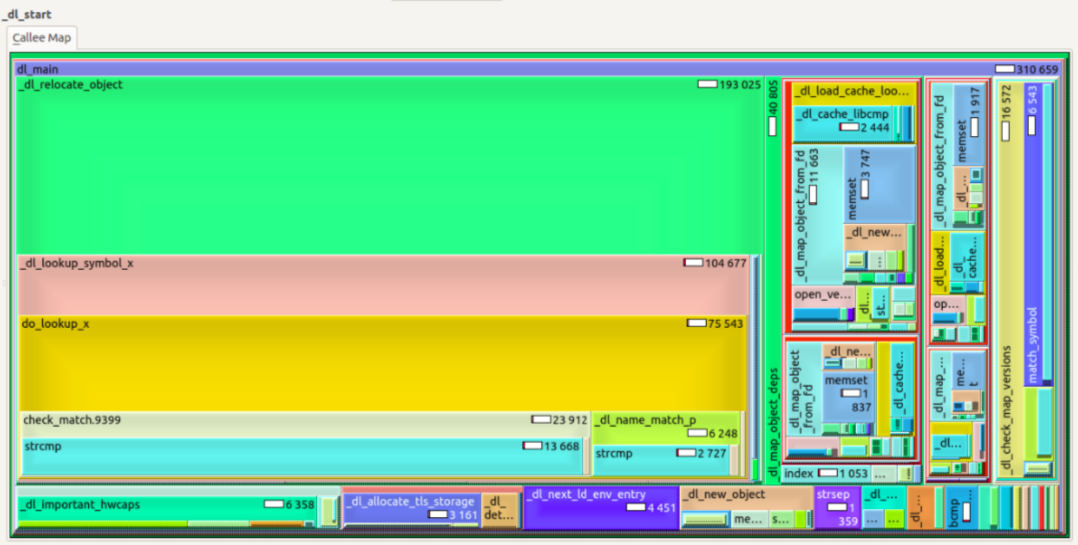
\includegraphics[scale=.6]{pic1.png}
\item cost (in terms of cycles) associated with the most expensive function calls.\\
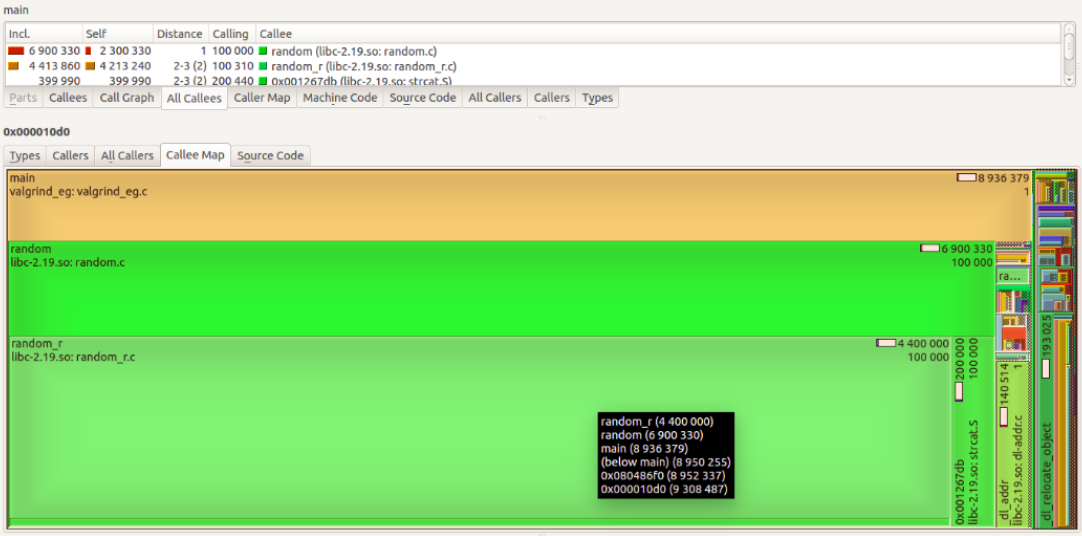
\includegraphics[scale=.6]{pic2.png}
\item cost (in terms of cycles) associated with pthread$\_$mutex$\_$lock.c and pthread$\_$mutex$\_$unlock.c\\
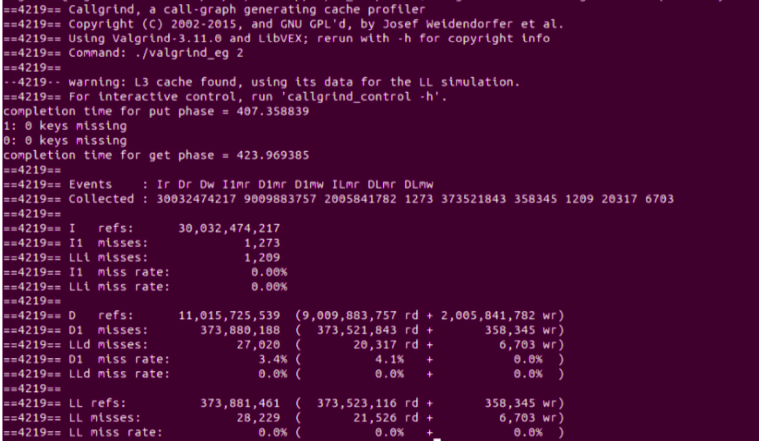
\includegraphics[scale=.6]{pic3.png}
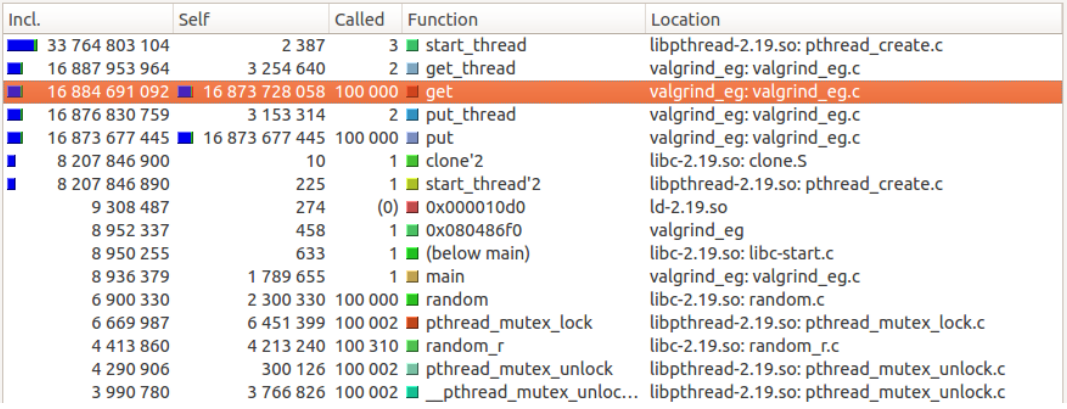
\includegraphics[scale=.6]{pic4.png}
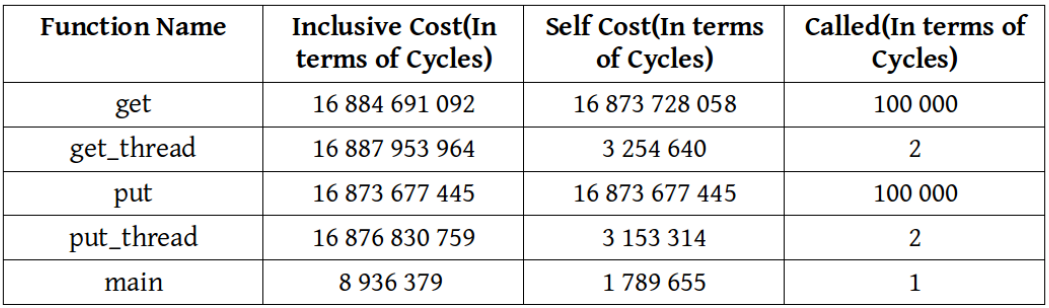
\includegraphics[scale=.6]{pic5.png}
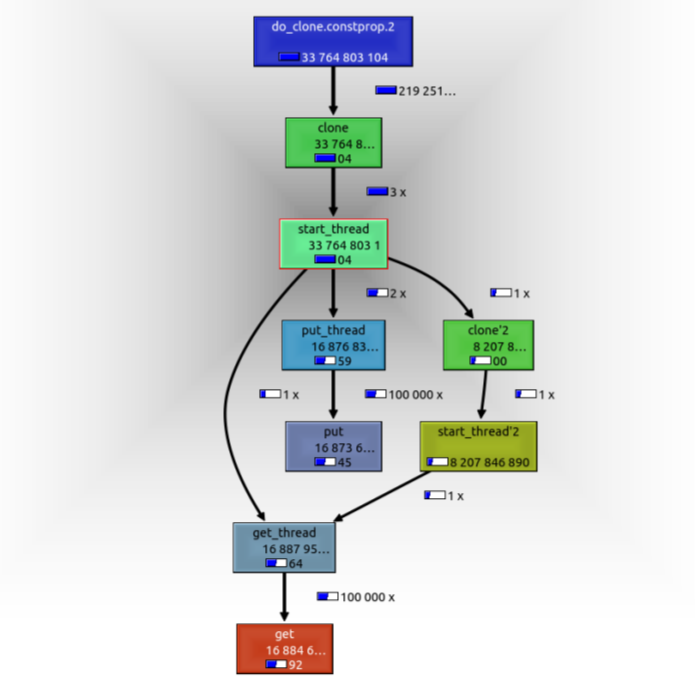
\includegraphics[scale=.6]{pic6.png}

\end{itemize}
\end{enumerate}

\end{document}